%% 03-Instrument_Data_Description.tex

\clearpage
\section{Instrument Data Description}
\label{sec:instrument_data_description}

METIS data uses the FITS format for both raw and product data
files. Raw frames are the unprocessed output of METIS instrument
observations, while product frames are the result of pipeline
processing.

All data files can be classified on the basis of sets of keywords
stored in the FITS headers. Association of raw frames to calibration
files is achieved by comparing keyword values.

\TODO{The following is taken verbatim from the PDR document,
  \cite{DRLS}. Updates are currently being discussed in the interface
  control document between ICS and PIP and will be ported here once
  finished. In particular the format for the N-band data from the new
  GeoSnap detector needs to be updated.}

\subsection{Raw data format}
\label{ssec:instrument_data_format}

All raw data files produced by METIS will be in FITS format and follow
ESO standards (\REQ{METIS-6081}, \REQ{METIS-6093}), in particular as
laid out in \cite{ESO-DICD}.

Data from the different subsystems (LM imager/spectrograph, NQ
imager/spectrograph, LM IFU) are always stored in separate files.
When more than one subsystem is recording data simultaneously, then
more than one FITS file is created by one observing template.

The LM and NQ imagers are single-chip sub-instruments, hence the
imaging data will appear in the primary HDU of the FITS file. The IFU
integral-field spectrograph consists of four chips, hence the FITS
file will consist of an empty primary data unit, whose header holds
information pertaining to the exposure as a whole, and four extension
units that hold the data from the four chips along with information
pertaining to each chip (such as world-coordinate system).

A template may produce several exposures, each of which consists of
NDIT subexposures (DITs). The exact definition of what constitutes an
``exposure'' or which and how many DITs will be save in a FITS file,
are still under discussion. The goal will be for a file to contain the
``smallest calibratable subset'' of DITs, for instance one cycle of
the chopping patters, or data taken in one nod position. Keeping files
small in this way allows the pipeline to process data even for cases
where observing blocks are only partially executed.

Where applicable, all the DITs belonging to an exposure may be saved
in a 3D-cube format. This is described in more detail for the various
observing modes in the following sections.

The raw data should include World Coordinate Systems based on the
telescope pointing, derotator angle and the design characteristics of
the telescope and instrument. Instrument-internal coordinates
(e.g.~angles of movable components inside METIS) will follow the
definition in \cite{METIS-coordinates} (\REQ{METIS-6070}).

The list of these FITS header keywords used by METIS is kept in
\cite{METIS-DID}.



%%%%%%%%%%%%%%%%%%%%%%%%%%%%%%%%%%%%%%%%%%%%%%%%%%%%%%%%%%%%%%%%%%%%%%%%%%%%%%%%

\subsection{LM-band Imager and Spectrograph}
\label{ssec:instrument_data_LM-IMG}

The LM-band imager is equipped with a $2\mathrm{k}\times2\mathrm{k}$
HAWAII2RG detector with a pixel scale of $5.47\,\mathrm{mas}$. A
number of rows and columns along the edges of the detector will be
masked (see Sect.~8.2 of \cite{DRLS}).

Grisms in the imager pupil wheel in conjunction with a number of slit
masks in the CFO focal plane provide low-resolution spectroscopy
covering the entire L~and M~bands, respectively, with $R\ga 1400$.

The basic templates for LM-band imaging are
(\cite{METIS-operational_concept}, \cite{METIS-template_manual}):
\begin{itemize}
\item \lstinline{METIS_img_lm_obs_AutoJitter}
\item \lstinline{METIS_img_lm_obs_GenericOffset}
\item \lstinline{METIS_img_lm_obs_FixedSkyOffset}
\end{itemize}

Each of these templates moves the target position between exposures,
either using the internal (CFO-PP2) chopper or telescope offsets, and
takes an exposure at each position, consisting of subintegrations
defined by DIT and NDIT. Depending on the setting of a Boolean
template parameter (\FITS{DET CUBE MODE}), all DITs are stored as
layers of 3D cube, or a co-added frame is stored as a 2D image. The 3D
cube or 2D image are written out in the primary HDU of the FITS file.

The header of the FITS file will contain all information that pertains
to the exposure. This should include information about the position of
the internal chopper (\FITS{SEQ.CFO.CHOP.POSANG},
\FITS{SEQ.CFO.CHOP.THROW}), the telescope offsets (\FITS{SEQ OFFSET1},
\FITS{SEQ OFFSET2}) and the characterisation of the observation as
\FITS{OBJECT} or \FITS{SKY} (in \FITS{DPR.TYPE}).

Similar considerations apply to the spectroscopic and coronagraphic
templates, where pointing offsets are however restricted by the slit
or coronagraphic masks.

%%
%%\begin{center}
%%\begin{table}
%%  \caption[LM\_IMG data keywords]{Columns foreseen for the LM
%%    imager/spectrograph FITS files.}
%%\label{tab:lm_img_colums}
%%\begin{tabular}{|l|l|p{10cm}|}
%%  \hline
%%  \textbf{Column} & \textbf{Format}      & \textbf{Description}                                       \\
%%  \hline\hline
%%  TIME            & long integer         & Time since start of this observation in milliseconds (TBD) \\
%%  \hline
%%  OBSTYPE         & OBJ or SKY           & Exposure on target or on sky?                              \\
%%  \hline
%%  NODDIST         & float (arcsec)       & Nodding distance from reference position                   \\
%%  \hline
%%  CHOPPOS         & $0\dots 360$         & Chopper position angle                                     \\
%%  \hline
%%  CHOPTHROW       & float (mas)          & Chopper distance from reference position                   \\
%%  \hline
%%  CHOPPER         & string               & Flag specifying the position of the internal chopper       \\
%%  \hline
%%  IMAGE           & 2k$\times$2k integer & Raw detector image                                         \\
%%  \hline
%%\end{tabular}
%%\end{table}
%%\end{center}
%%%%%%%%%%%%%%%%%%%%%%%%%%%%%%%%%%%%%%%%%%%%%%%%%%%%%%%%%%%%%%%%%%%%%%%%%%%%%%%%

\subsection{N-band Imager and Spectrograph}
\label{ssec:instrument_data_N-IMG}

The N-band imager is equipped with a $2\mathrm{k}\times 2\mathrm{k}$
GeoSnap detector with a pixel scale of $6.8\,\mathrm{mas}$. A number
of rows and columns along the edges of the detector will be masked.

A grism in the imager pupil wheel in conjunction with a number of slit
masks in the CFO focal plane provide low-resolution spectroscopy in
the N~band with $R\ga 400$.

Subtraction of the thermal background in the N~band will be done using
chopping at a few Hertz using the internal chopper and regular nodding
using telescope offsets. The basic templates for N~imaging are
\begin{itemize}
\item \lstinline{METIS_img_n_obs_AutoChopNod}
\item \lstinline{METIS_img_n_obs_GenericChopNod}
\end{itemize}

At each nod position, a series of exposures are taken at alternating
chop positions. Depending on the setting of the template parameter
\FITS{DET CUBE MODE}, all exposures are stored as layers of a 3D cube
or they are precombined in a 2D image. Another chop cycle is then
taken at another nod position, and so on. Whether separate nod
positions are stored as individual FITS files or as extension units of
a single FITS file remains to be determined. As explained in
Sect.~\ref{ssec:instrument_data_format}, there is a preference for
small FITS files containing minimal calibratable subsets of DITs.

The primary header of the FITS file will contain all information that
pertains to the chop cycle or the sequence of chop/nod cycle. The
headers of the individual files or extensions will allow unique
determination of the chop/nod positions.

%%\begin{center}
%%\begin{table}
%%\caption[NQ\_IMG data keywords]{Columns foreseen for the NQ imager/spectrograph FITS files.}
%%\label{tab:nq_img_colums}
%%\begin{tabular}{|l|l|p{10cm}|}
%%  \hline
%%  \textbf{Column} & \textbf{Format}      & \textbf{Description}                                       \\
%%  \hline\hline
%%  TIME            & long integer         & Time since start of this observation in milliseconds (TBD) \\
%%  \hline
%%  OBSTYPE         & OBJ or SKY           & Exposure on target or on sky?                              \\
%%  \hline
%%  NODDIST         & float (arcsec)       & Nodding distance from reference position                   \\
%%  \hline
%%  CHOPPOS         & $0\dots 360$         & Chopper position angle                                     \\
%%  \hline
%%  CHOPTHROW       & float (mas)          & Chopper distance from reference position                   \\
%%  \hline
%%  CHOPPER         & string               & Flag specifying the position of the internal chopper       \\
%%  \hline
%%  IMAGE           & 1k$\times$1k integer & Raw detector image                                         \\
%%  \hline
%%\end{tabular}
%%\end{table}
%%\end{center}

%%%%%%%%%%%%%%%%%%%%%%%%%%%%%%%%%%%%%%%%%%%%%%%%%%%%%%%%%%%%%%%%%%%%%%%%%%%%%%%%

\subsection{LM-band Integral Field Unit}
\label{ssec:instrument_data_IFU}

METIS will contain an image slicing integral-field unit (IFU) for
high-resolution spectroscopy in L- and M-band ($R\approx
100,000$).
This used to be referred to as ``\ac{LMS}'', but will be refered to as ``\ac{IFU}'' to prevent confusion.

The IFU is equipped with a $2\times2$ mosaic of HAWAII2RG detectors
separated by small gaps. A number of rows and columns along the edges
of the detector will be masked (see Sect.~8.2 of \cite{DRLS}).

In the nominal mode, the field will be resolved into 28 spatial slices
covering a field of view of $0.93\times0.58\,\mathrm{arcsec^{2}}$.
The slit width (i.e.\ the across-slice pixel scale) is
$20.7\,\mathrm{mas}$; the along-slice pixel scale is
$8.2\,\mathrm{mas}$. Spectrally, the slices span a short wavelength
range of width $37\,\mathrm{nm}$ and $70\,\mathrm{nm}$, depending on
the central wavelength setting, which is selected by rotation of the
echelle grating.

The extended mode provides a larger wavelength range coverage at the
expense of a reduced field of view. The dispersed two-dimensional
image from the pre-disperser is spectrally sliced, resulting in six
non-overlapping wavelength subranges (selected by the echelle angle)
onto the detector, each with three spatial slices.

The layout of spectra on the detector array in the nominal and
extended modes is shown in the left and right panels of
Fig.~\ref{fig:IFU_detector_layout}, respectively.

\begin{figure}[ht]
  \centering
  \resizebox{0.495\textwidth}{!}{%
    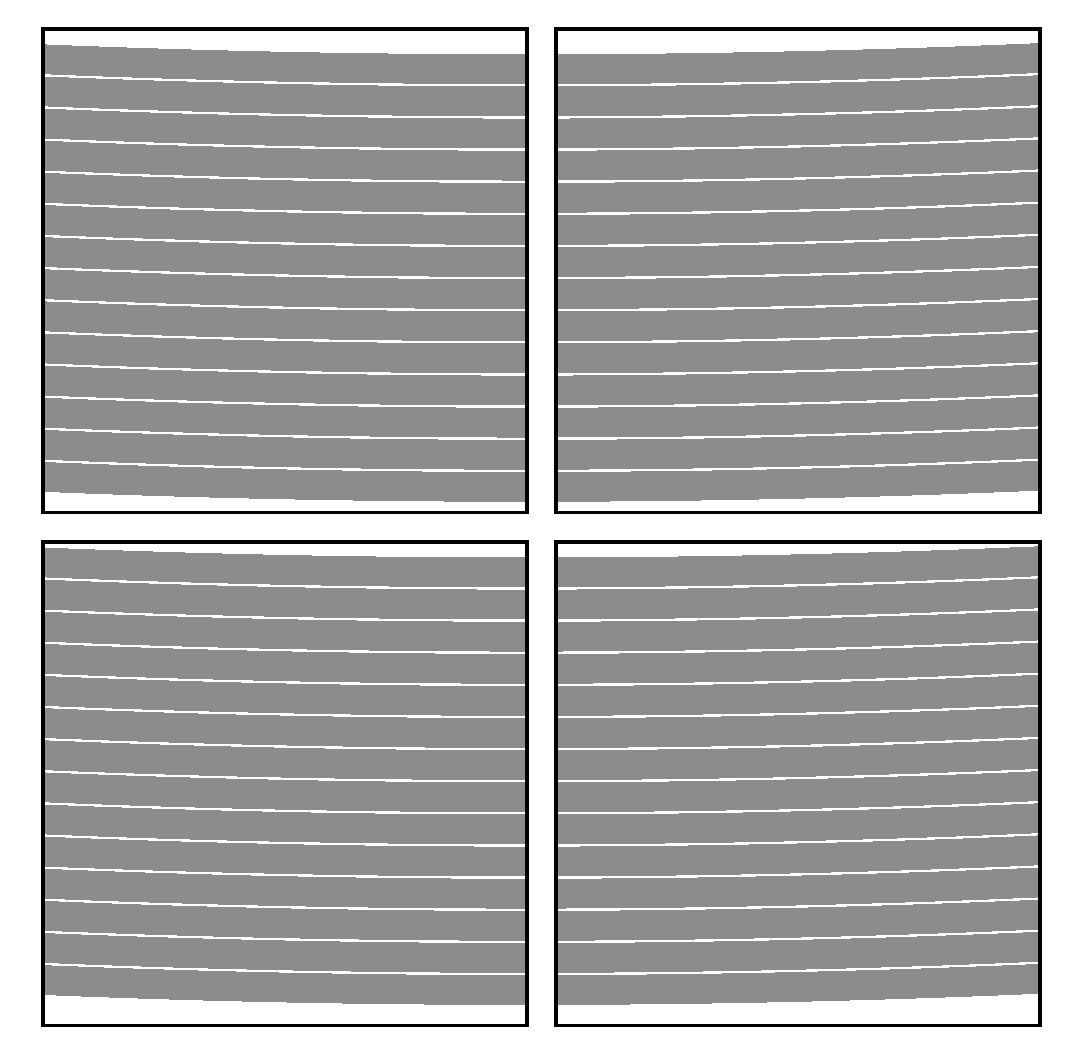
\includegraphics{LMS_detector_layout_normal_tikz}}\hfill
  \resizebox{0.495\textwidth}{!}{%
    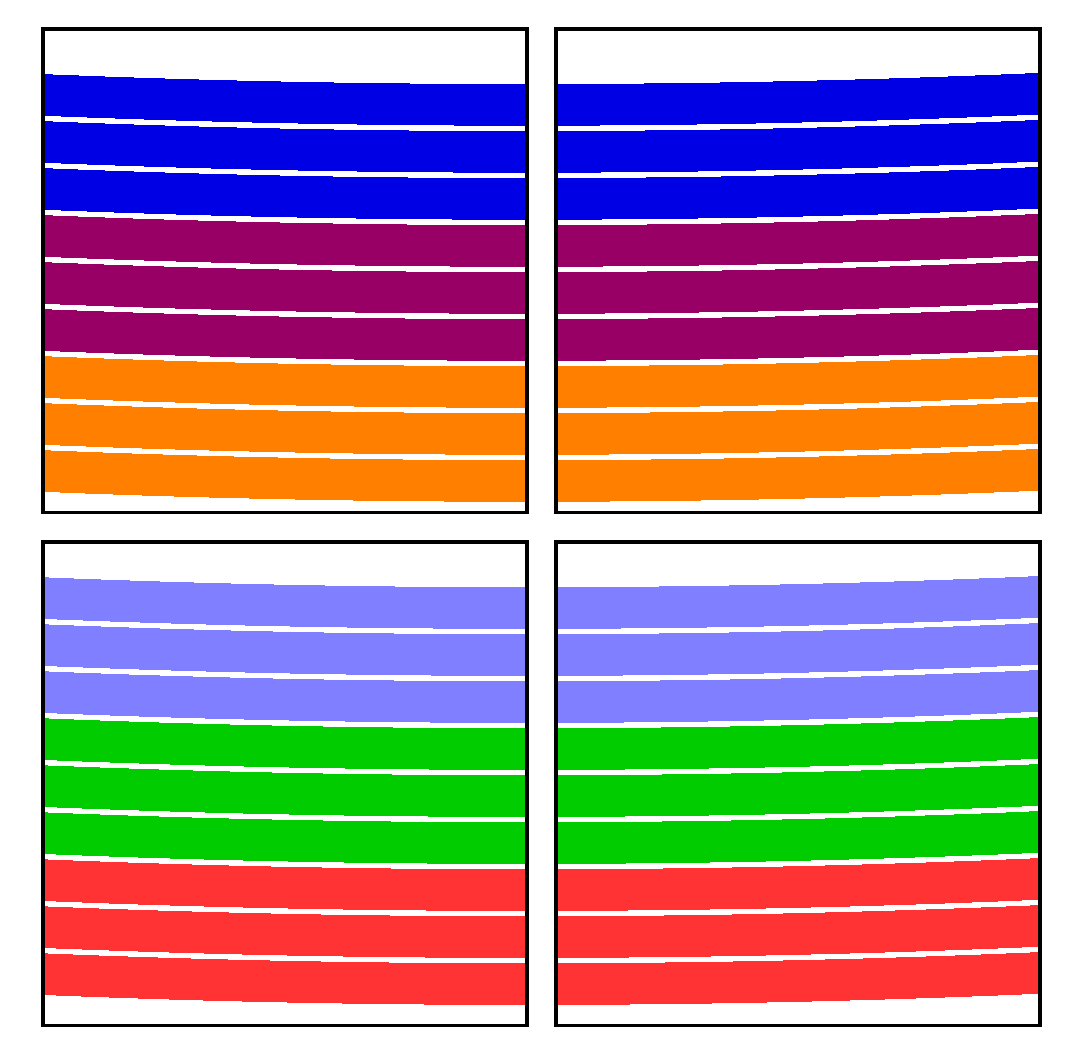
\includegraphics{LMS_detector_layout_extended_tikz}}
  \caption[IFU detector layout]{Layout of the IFU detector mosaic
    in the nominal (left) and extended (right) modes. The dispersion
    direction is horizontal. In the nominal mode, all 28 slices cover
    the same wavelength range. In the extended mode, slices marked by
    the same colour cover the same wavelength ranges, while the
    wavelength ranges of the six groups of slices each are not
    contiguous. The position and curvature of the slices are
    indicative only. }
  \label{fig:IFU_detector_layout}
\end{figure}

The basic templates for LM integral-field spectroscopy are:
\begin{itemize}
\item \lstinline{METIS_ifu_obs_FixedSkyOffset}
\item \lstinline{METIS_ifu_obs_GenericOffset}
\end{itemize}
Both templates move the target position between exposures, using the
internal chopper or the telescope. At a given position a number of
exposures with DIT/NDIT are taken. Depending on the setting of the
template parameter \FITS{DET CUBE MODE} all the DITs may be stored as
layers of a 3D cube (burst mode) or co-added into a 2D image.

As the IFU contains an array of four detectors, there will be four
image or cube extensions in the FITS file for one exposure.

The primary header of the FITS file will contain all information that
pertains to the exposure. This will include information on the
position of the internal chopper, the telescope offsets, and the type
of observation (\FITS{DPR.TYPE=OBJECT} or \FITS{SKY}).

A typical sequence of IFU exposures will go through a series of
dispersion grating settings in order to fill gaps in the instantaneous
wavelength coverage (``spectral dithering''). Finally, the field will be
rotated by 90~degrees and the observing sequence repeated to permit
full image reconstruction
(cf.~Sect.~8.9 of \cite{DRLS}). The FITS header
information will ensure that the position of each exposure within this
complex sequence can be uniquely identified.

%%\begin{center}
%%\begin{table}
%%\caption[IFU data keywords]{Columns foreseen for the IFU FITS files.}
%%\label{tab:lms_colums}
%%\begin{tabular}{|l|l|p{10cm}|}
%%  \hline
%%  \textbf{Column} & \textbf{Format}      & \textbf{Description}                                       \\
%%  \hline
%%  TIME            & long integer         & Time since start of this observation in milliseconds (TBD) \\
%%  \hline
%%  OBSTYPE         & OBJ or SKY           & Exposure on target or on sky?                              \\
%%  \hline
%%  NODDIST         & float (arcsec)       & Nodding distance from reference position                   \\
%%  \hline
%%  CHOPPOS         & $0\dots 360$         & Chopper position angle                                     \\
%%  \hline
%%  CHOPTHROW       & float (mas)          & Chopper distance from reference position                   \\
%%  \hline
%%  CHOPPER         & string               & Flag specifying the position of the internal chopper       \\
%%  \hline
%%  IMAGE1          & 2k$\times$2k integer & raw image from detector 1                                  \\
%%  IMAGE2          & 2k$\times$2k integer & raw image from detector 2                                  \\
%%  IMAGE3          & 2k$\times$2k integer & raw image from detector 3                                  \\
%%  IMAGE4          & 2k$\times$2k integer & raw image from detector 4                                  \\
%%  \hline
%%\end{tabular}
%%\end{table}
%%\end{center}


\subsection{File classification keywords}
\label{ssec:file_classification_keywords}

\TODO{This section will contain the list of files with the values of
  kewords \FITS{DPR.CATG}, \FITS{DPR.TYPE}, \FITS{DPR.TECH}, \FITS{DO
    Category} in accordance with \cite{ESO-DICD}.}

%%%%%%%%%%%%%%%%%%%%%%%%%%%%%%%%%%%%%%%%%%%%%%%%%%%%%%%%%%%%%%%%%%%%%%%%%%%%%%%%
\subsection{Reduced data format}
\label{ssec:reduced_data_format}

All data products, both intermediary and final ones, will be provided in FITS format. Final data products will be saved according to \cite{ESO-products_standard}. This fulfills \REQ{METIS-6061} and \REQ{METIS-6082}.

The list of data products can be found in Ch.~\ref{sec:drl_data_structures}.

% THE END
%%%%%%%%%%%%%%%%%%%%%%%%%%%%%%%%%%%%%%%%%%%%%%%%%%%%%%%%%%%%%%%%%%%%%%%%%%%%%%%%

%%% Local Variables:
%%% TeX-master: "METIS_DRLD"
%%% End:
